%%%%%%%%%%%%%%%%%%%%%%%%%%%%%%%%%%%%%%%%%
% "TRIBES/Nedap manual/experience report
% LaTeX Template
% Version 1.0 (2018/11/27)
%
%
% Original author:
% Marc Pichel (marc.pichel@nedap.com)
%
%This guide is here to help new people become more adquainted
%
% Important note:
% If you add any style documents, mention them here
%%%%%%%%%%%%%%%%%%%%%%%%%%%%%%%%%%%%%%%%%

%----------------------------------------------------------------------------------------
%	PACKAGES AND OTHER DOCUMENT CONFIGURATIONS
%----------------------------------------------------------------------------------------

\documentclass[11pt,a4paper,sans]{report} % Font sizes: 10, 11, or 12; paper sizes: a4paper, letterpaper, a5paper, legalpaper, executivepaper or landscape; font families: sans or roman. I used 'article' class since this is a short report, but feel free to edit if this is ever expanded into an actual manual ;)

\usepackage{subcaption}
\usepackage{graphicx}
\usepackage{hyperref} % Allows hyperlink references in text, see interwebs for use
%\usepackage[...]{hyperref} % Needed for some style 
\usepackage[scale=0.75]{geometry} % Reduce document margins


\begin{document}

%----------------------------------------------------------------------------------------
%	SHORT MANUAL (English - feel free to add a dutch equivalent to this document)
%----------------------------------------------------------------------------------------

\title{Tribes' flex-work places for Ned(ummies)appers}
\author{Marc Pichel}
\date{\today}
\maketitle

\tableofcontents

\chapter{Intro}

Imagine you are heading out after an Onsbijtje, visiting friends/family, Couchsurfing or travelling through the non-eastern part of the Netherlands for other reasons, and you would like to kill a few work hours in a place with the following:
\begin{itemize}
	\item coffee or tea 
	\item a desk
	\item power
	\item shelter
\end{itemize}
but your host or the train stations are not adequate. Then the Tribes flex-workplace is a great alternative thanks to the Nedap partnership! (I am not getting paid by Nedap or Tribes to say this, it's true.) That said, I was missing some information on the Tribes visiting process, so made this guide of sorts out of laziness.

The other reason for this guide is to keep track of which flex-work places in which towns are the best (most comfortable), based on my/our own experience. This will come back in the final chapter. It might also make it easier to meet up at a work place outside Nedap with other Nedappers whether they are on a (business) trip or cautiously leaving `De Achterhoek' to explore the rest of the world. \#YOLO

\section{Tribes?}
It's just a cool co-working spot like WeWork, but with a theme of tribes from all around the world. If you are not sure where to find a Tribes work place, have a look \href{https://www.tribes.world/en/locations-listing-simple}{\textbf{\emph{here}}}.

\section{That's cool, but how much does it cost?}
Nothing. It's free as long as Nedap has a partnership with Tribes! I have no clue who is responsible for this :)

\chapter{Awesome, but how do I get in as Nedapper?}
In principle it is very straightforward: Ask at the front desk and thou shall receive. However, I did encounter a few bumps in my first experience at the Oval Tower office which might help you along the way and lower the anxiety threshold for visiting Tribes in general. There are basically 3 steps you need to go through to get access to a desk, coffee, shelter and unlimited (electrical) power:
\begin{enumerate}
	\item Find a nearby Tribes location.
	\item Tell someone at the frontdesk that you are from Nedap.
	\item Receive a visitor day-pass (access card) for general entrance and Tribes area.
\end{enumerate}
    
There are some requirements for each step:

\begin{enumerate}
	\item Location - Internet.
	\item Eligibility for a daypass - (Your) valid ID and Nedap card.
	\item Day-pass - Needs to be handed in at the end of the day (usually 18:00).
\end{enumerate}

If all went well, you should receive a Visitor Pass similar to figure \ref{fig.daypass} and get a setup similar to figure \ref{fig.coffeeandpower}. Well done!

\begin{figure}[htp]
\begin{subfigure}{.49\textwidth}
  \centering
  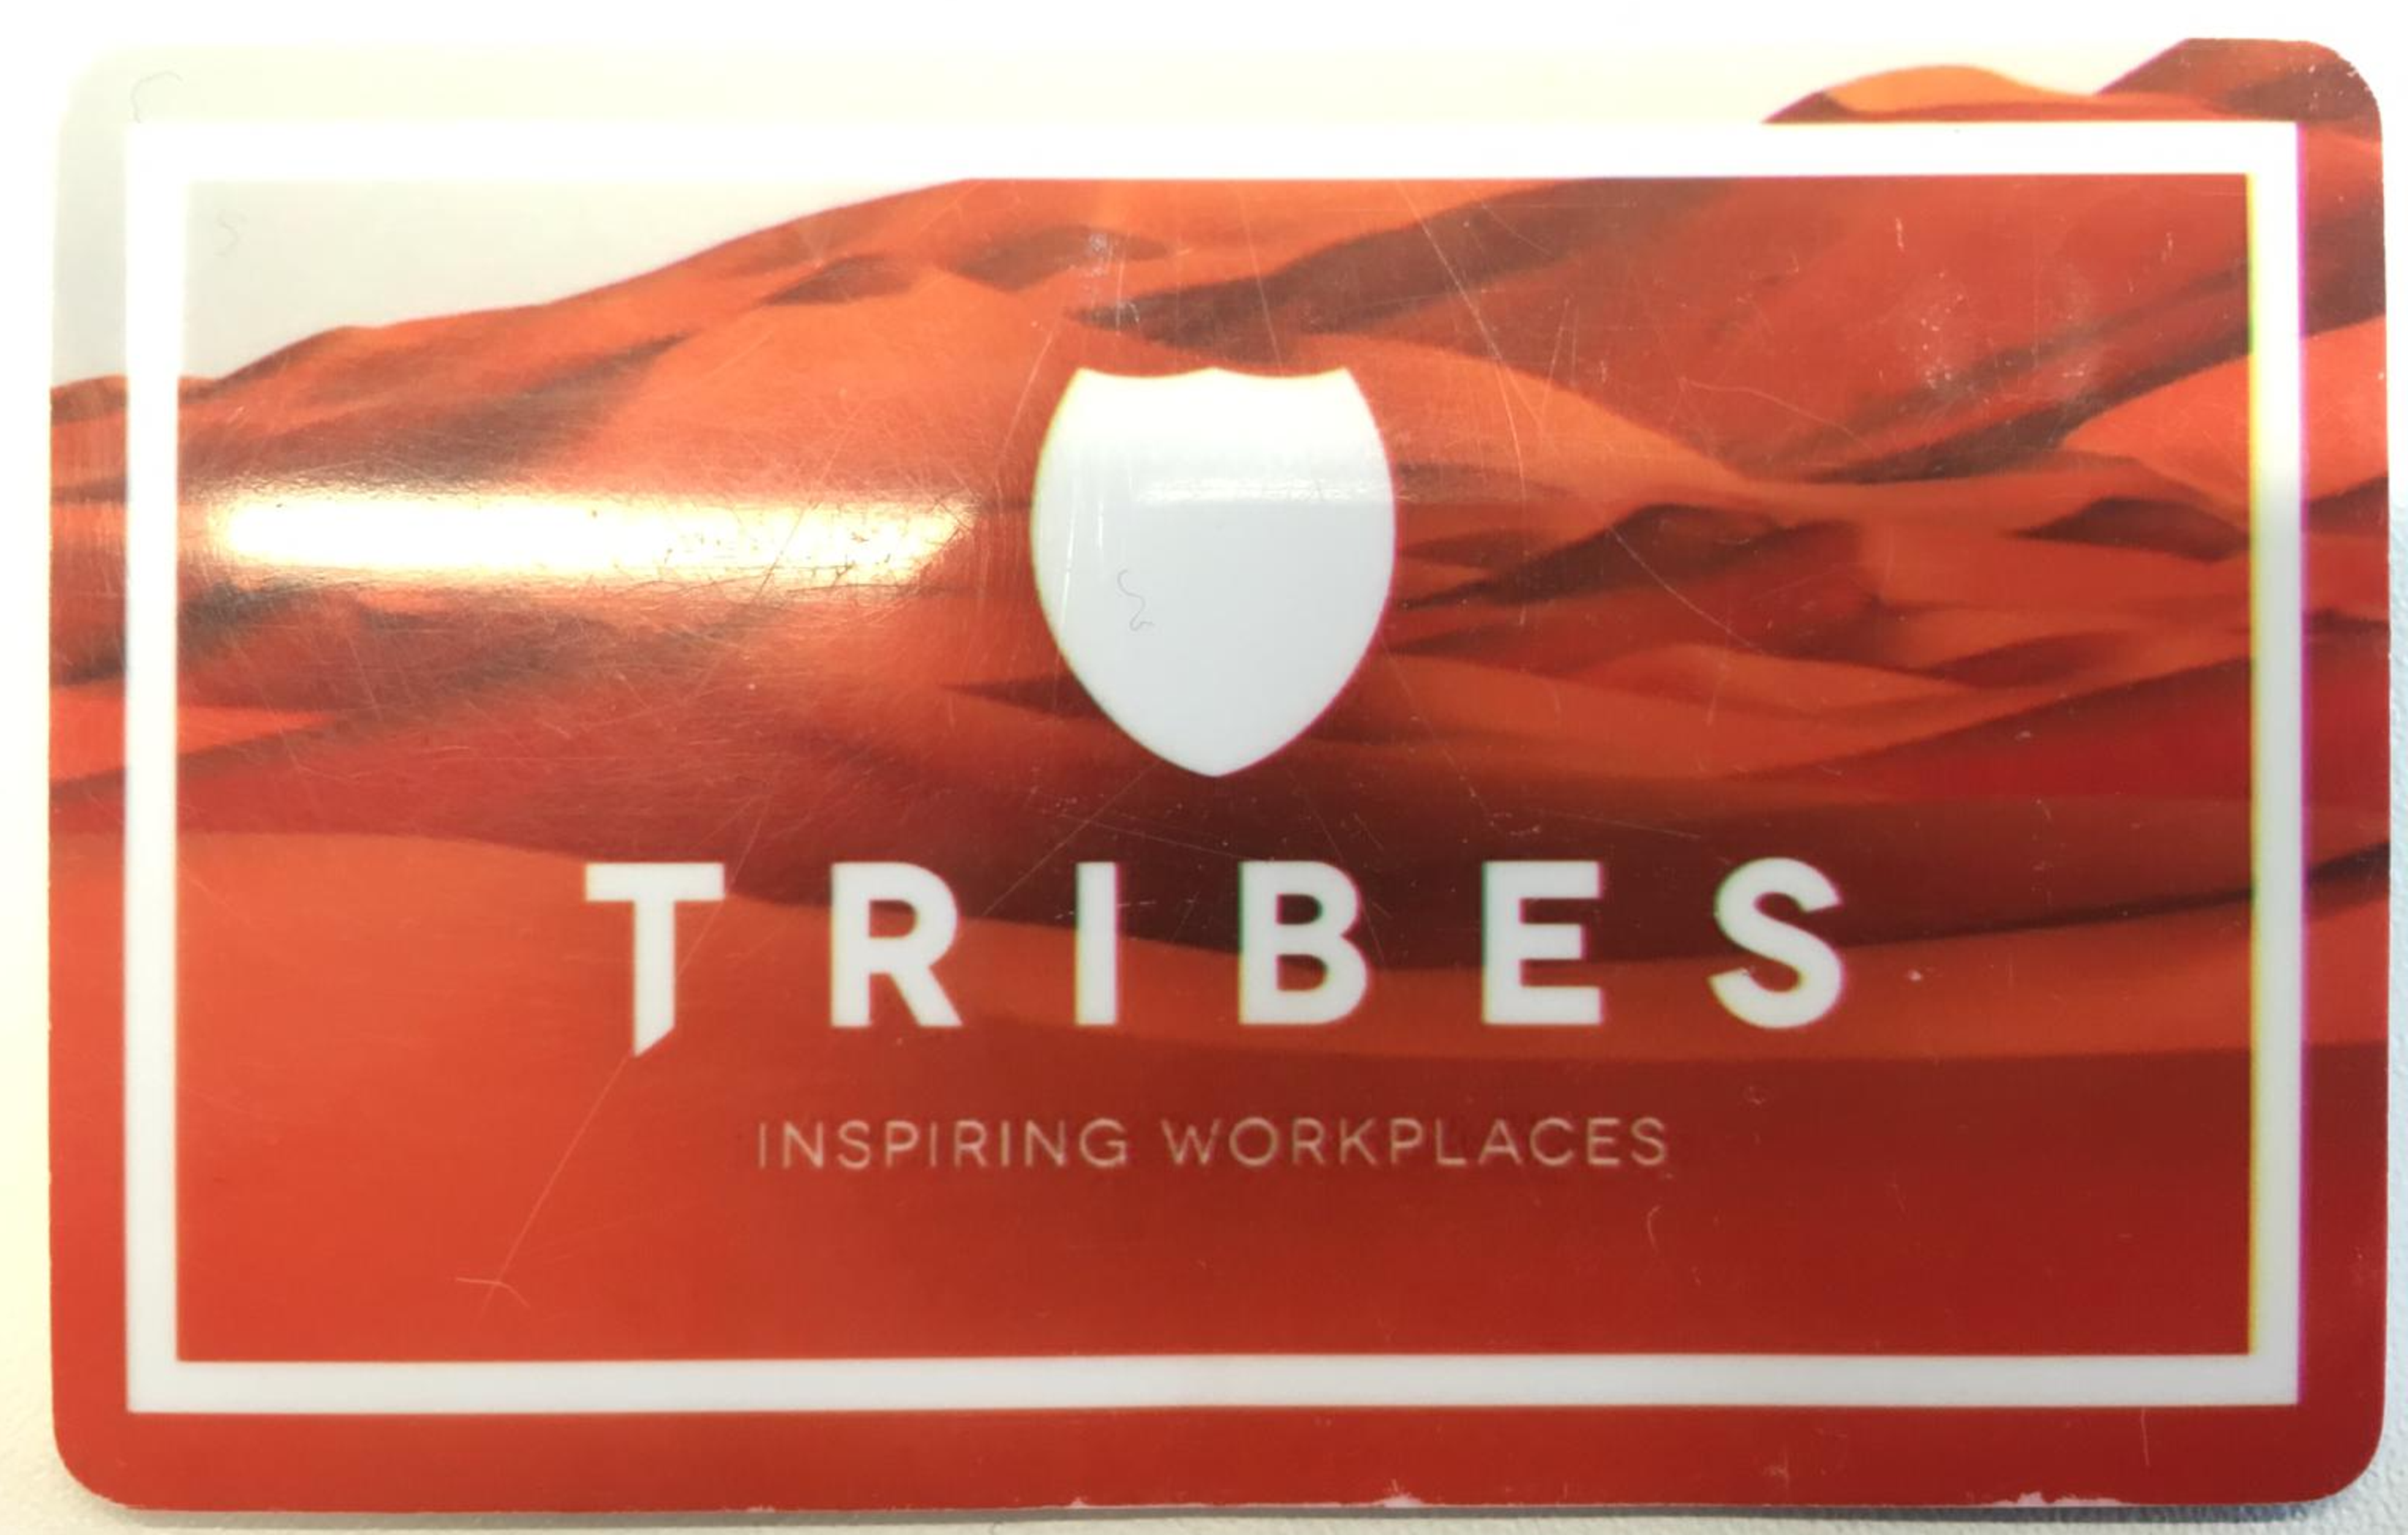
\includegraphics[width=1.0\linewidth]{images/amsovaltower/pasvoorkant}
  \caption{Frontside.}
  \label{fig.passfront}
\end{subfigure}%
\begin{subfigure}{.49\textwidth}
  \centering
  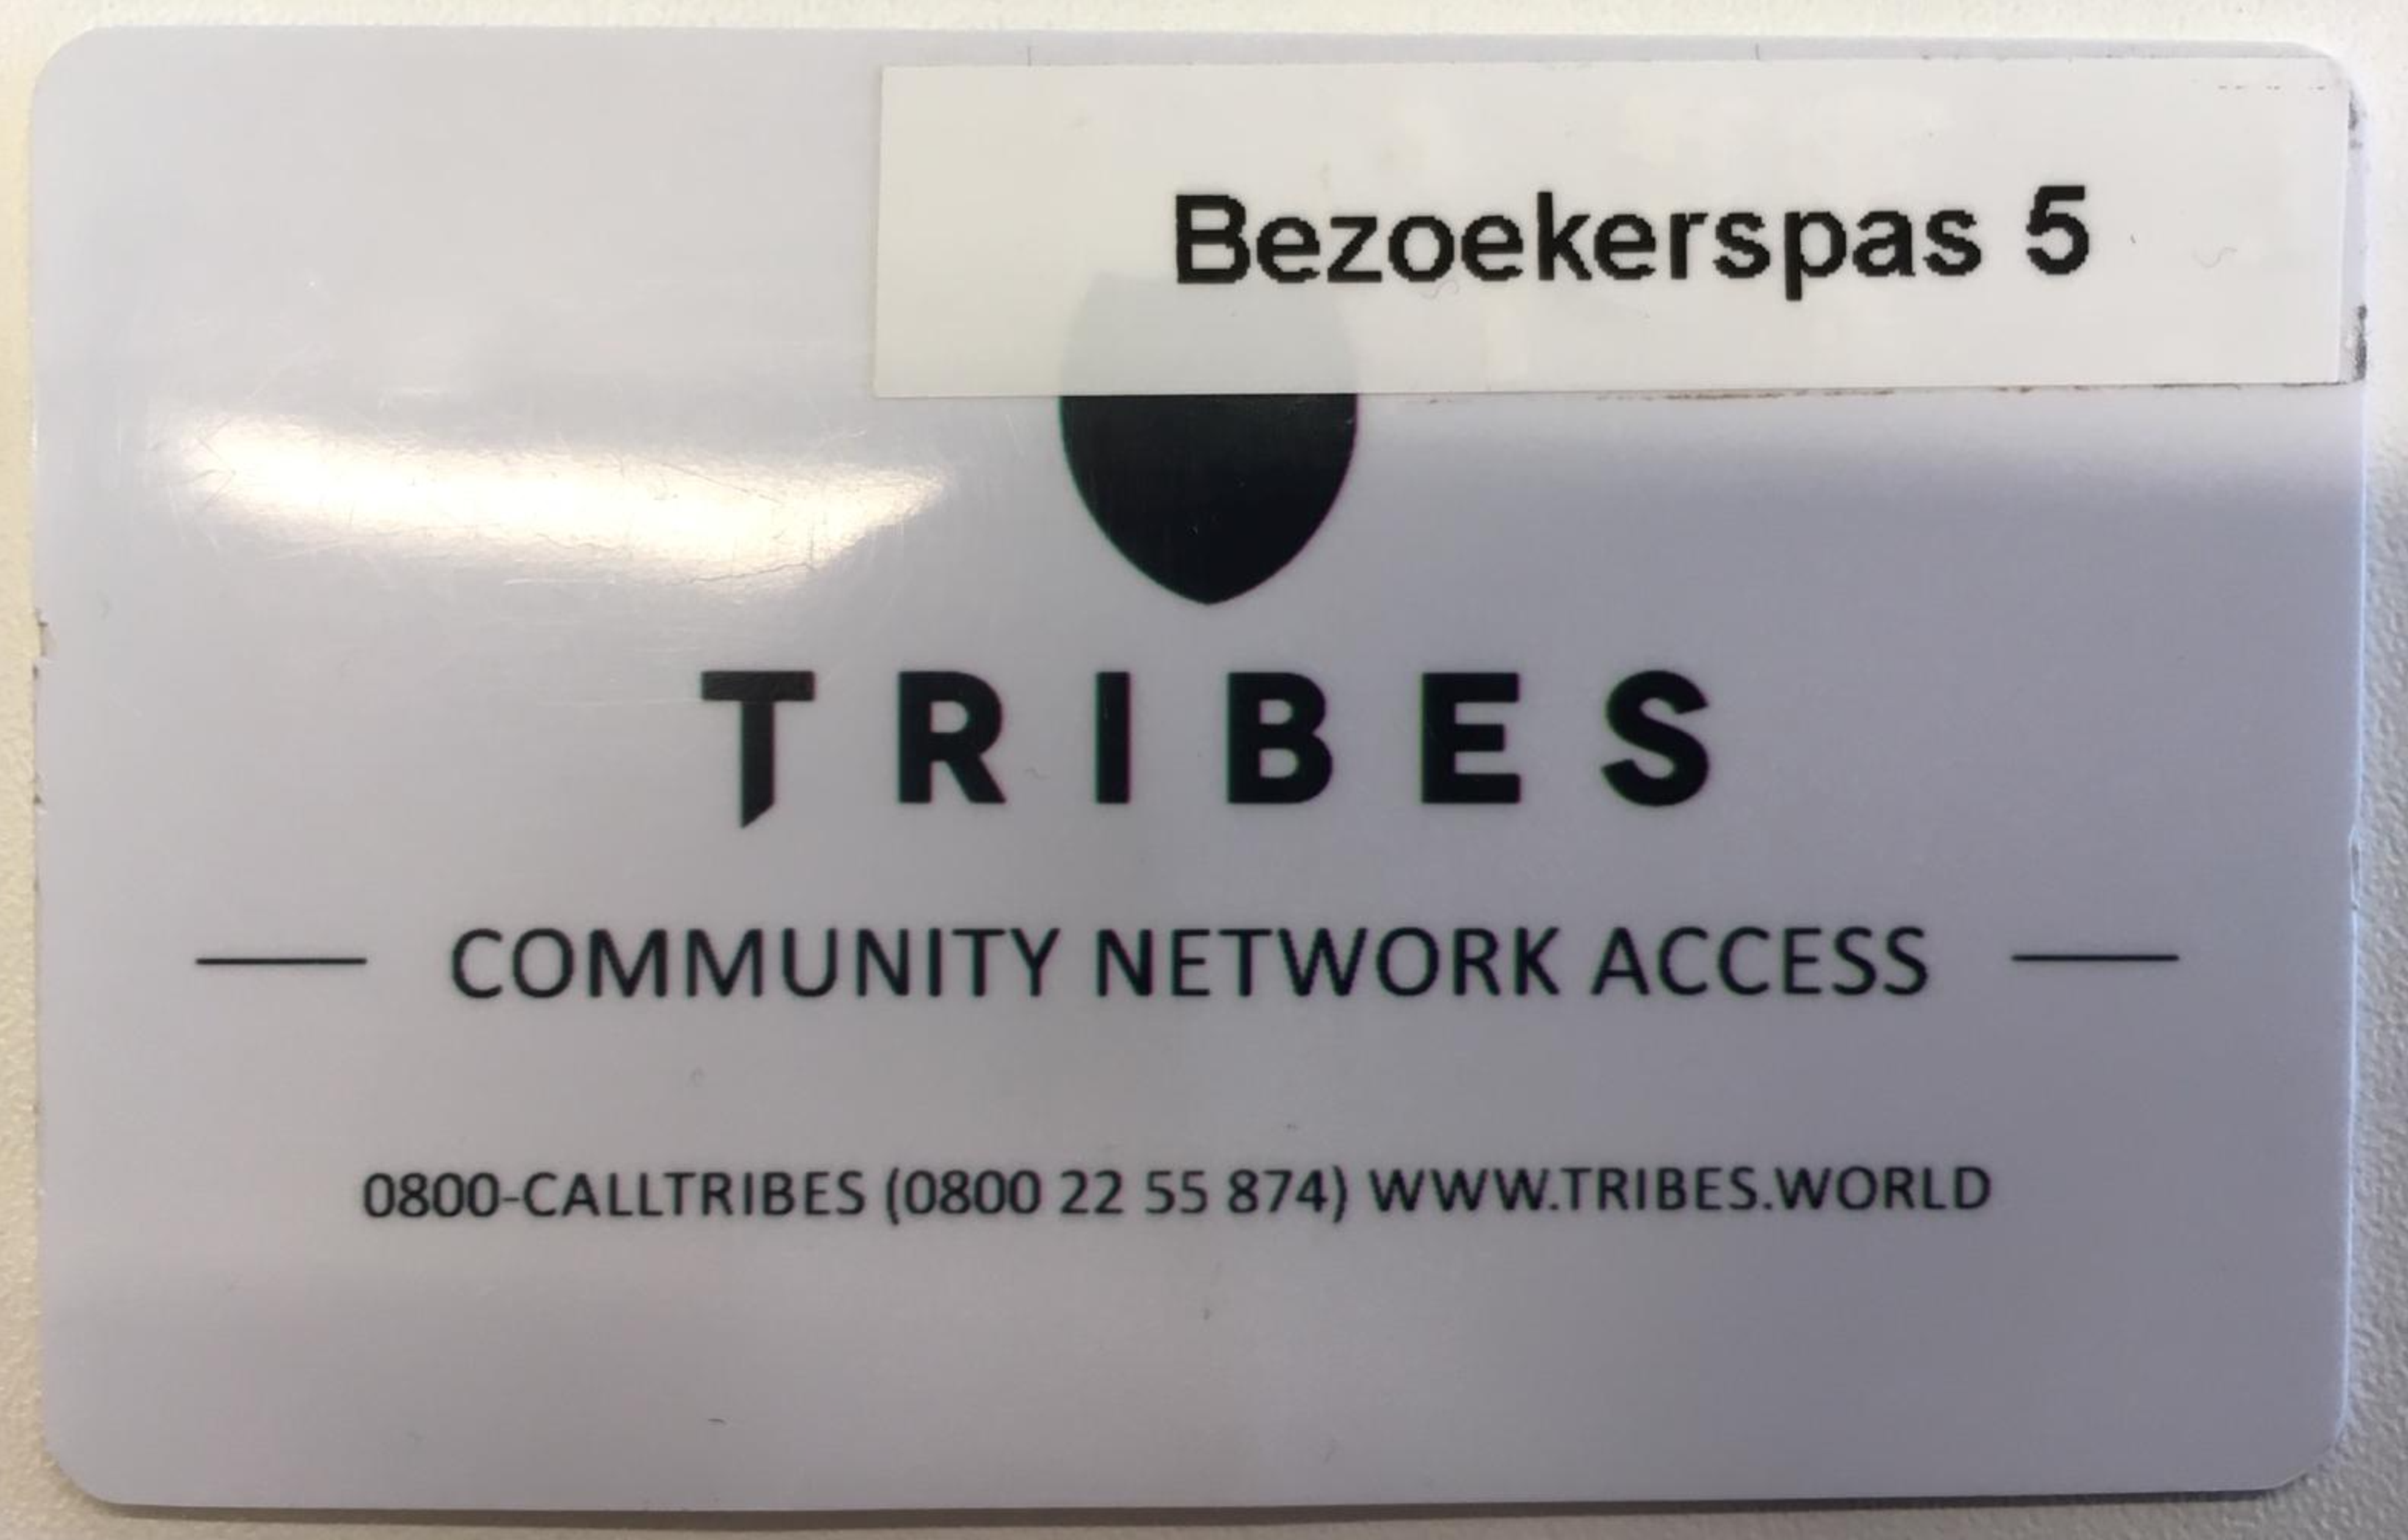
\includegraphics[width=1.0\linewidth]{images/amsovaltower/pasachterkant}
  \caption{Backside}
  \label{fig.passback}
\end{subfigure}
\caption{The 'Visitor Daypass'.}
\label{fig.daypass}
\end{figure}

\begin{figure}[htp]
	\centering
		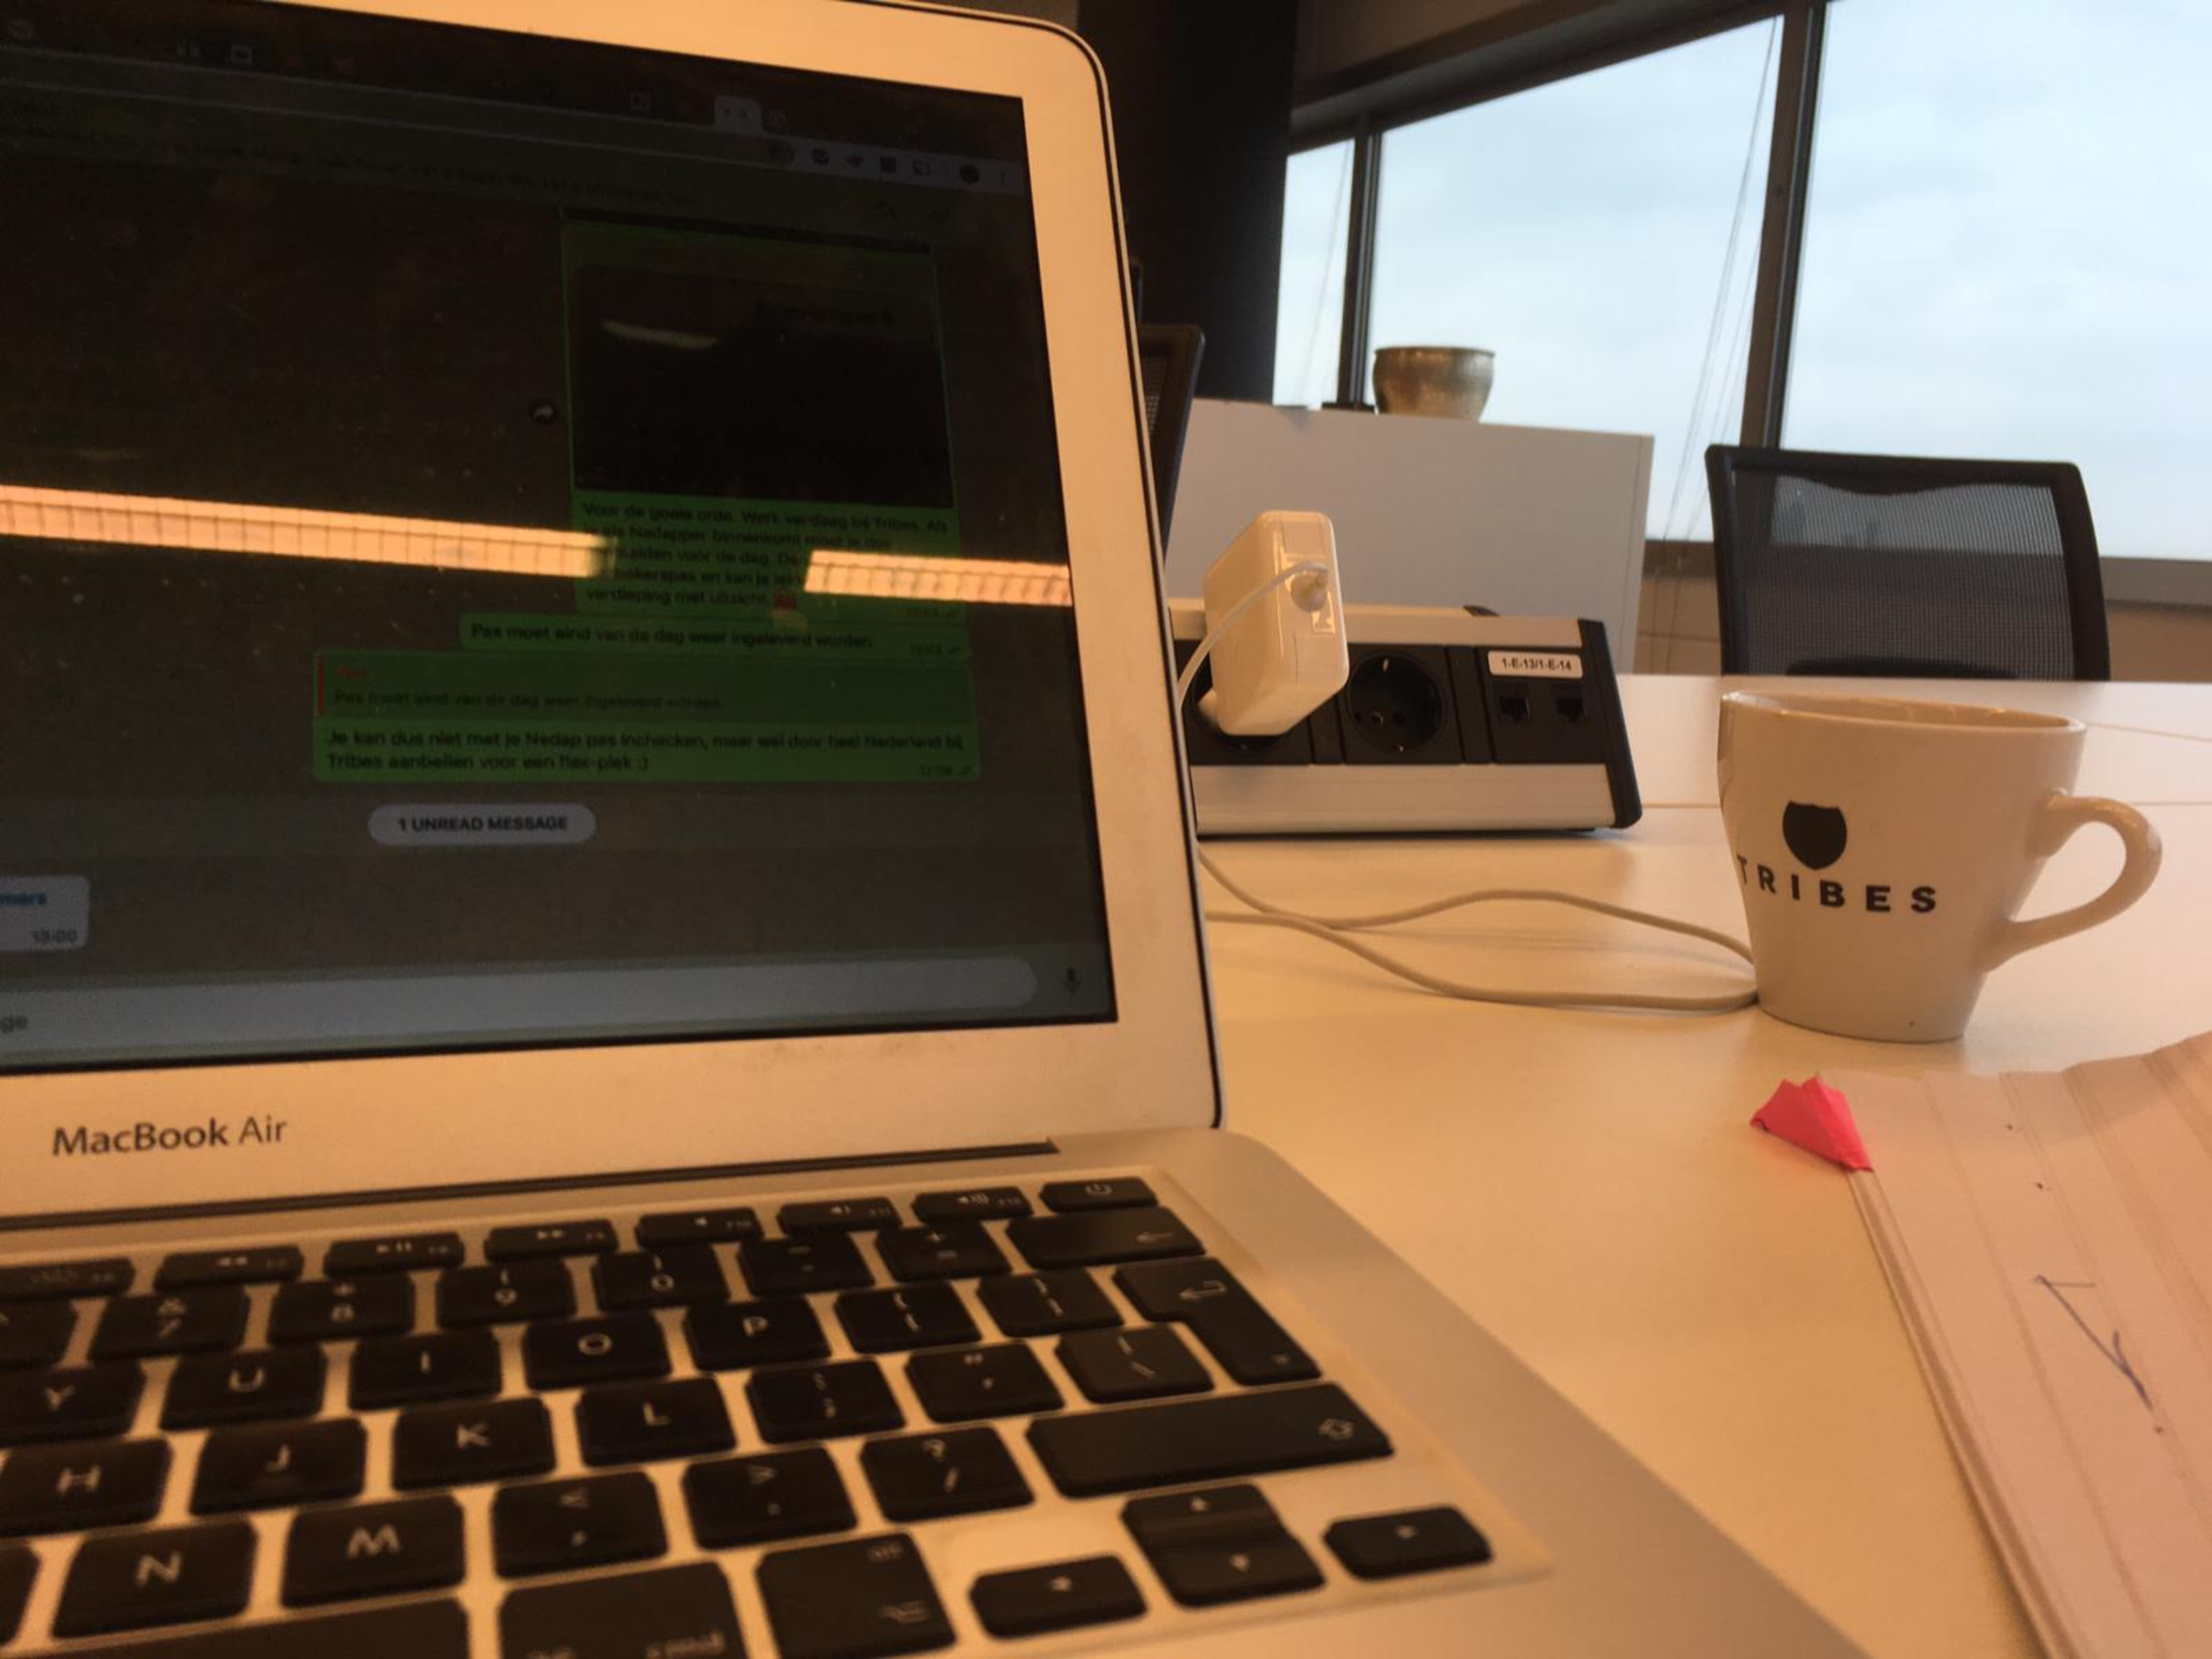
\includegraphics[width=1.0\linewidth]{images/amsovaltower/koffieenstroom}
	\caption{You should now be able to get to work!}
	\label{fig.coffeeandpower}
\end{figure}

\chapter{Field reports}

If anyone else is interested, we can populate this chapter with stories, tips, hints, etc. of specific locations. Think practical stuff like logistics, special elevators, places to grab (decent) food nearby or sights to see in case of serendipitous work-citytrip.

\section{Amsterdam, The Oval Tower}
The Oval Tower is a 5 minute (10 minutes if you hate exercise) walk from the Amsterdam Bijlmer Arena station. From figure \ref{fig.ovaltower} you can expect a view like \href{https://youtu.be/6oQ-9Qe8CHE}{\textbf{\emph{this}}} from the 11th floor. They told me it was warmer here than on the 15\textsuperscript{th} - not tested. Will update.

\begin{figure}[hpt]
	\centering
	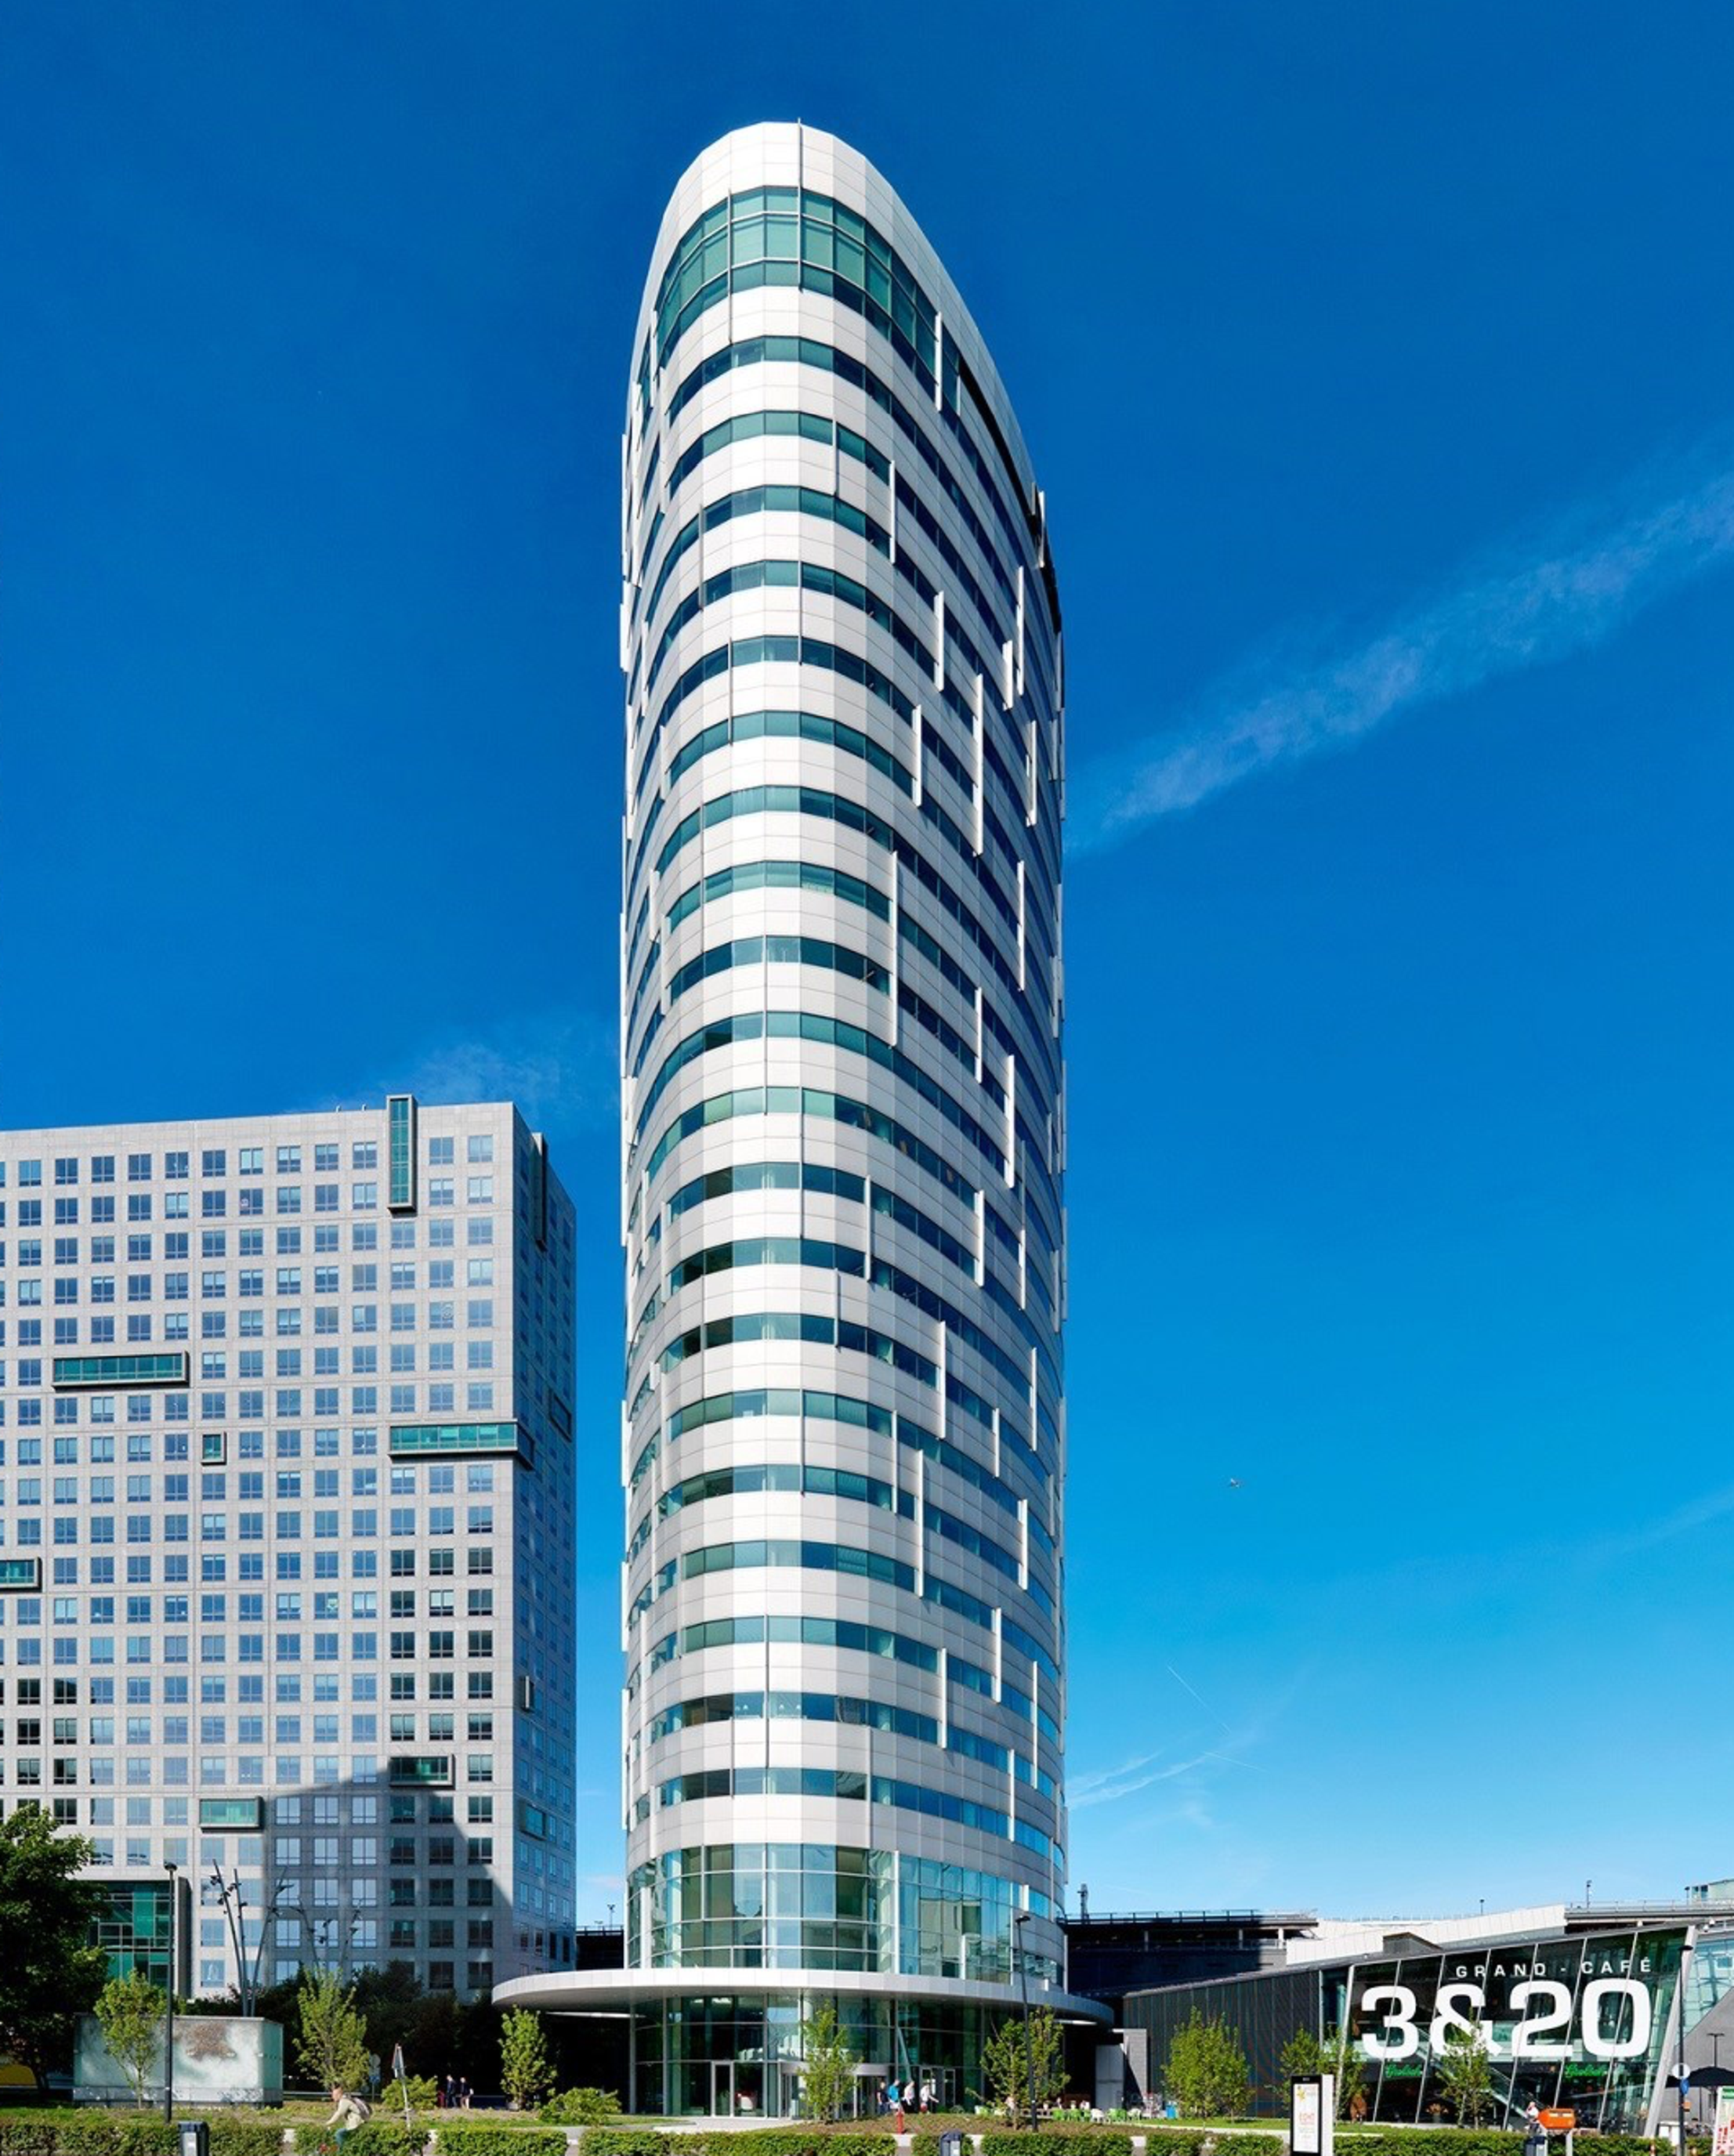
\includegraphics[width=0.5\linewidth]{images/amsovaltower/ovaltower}
	\caption{Probably the summer view.}
	\label{fig.ovaltower}
\end{figure}

They have a very interesting elevator policy: Press the floor button \textbf{before} entering the elevator, since there are none on the inside. I found out after I rushed into one with a group full of people. We had a laugh at my incompetence :)

Added by Jeroen Harmsen: I've worked at Amsterdam Arena: to go to the 15th floor, you first have to go to the 11th floor as the elevator doesn't stop at 15. Then change elevator and go to the 15th floor (same going the ground floor). Meeting rooms are 28.35 per person per morning/afternoon (so 56 euro's for a 2 person meeting), incl. coffee, tea, etc.

\begin{figure}[hpt]
	\centering
	\label{fig.elevator}
		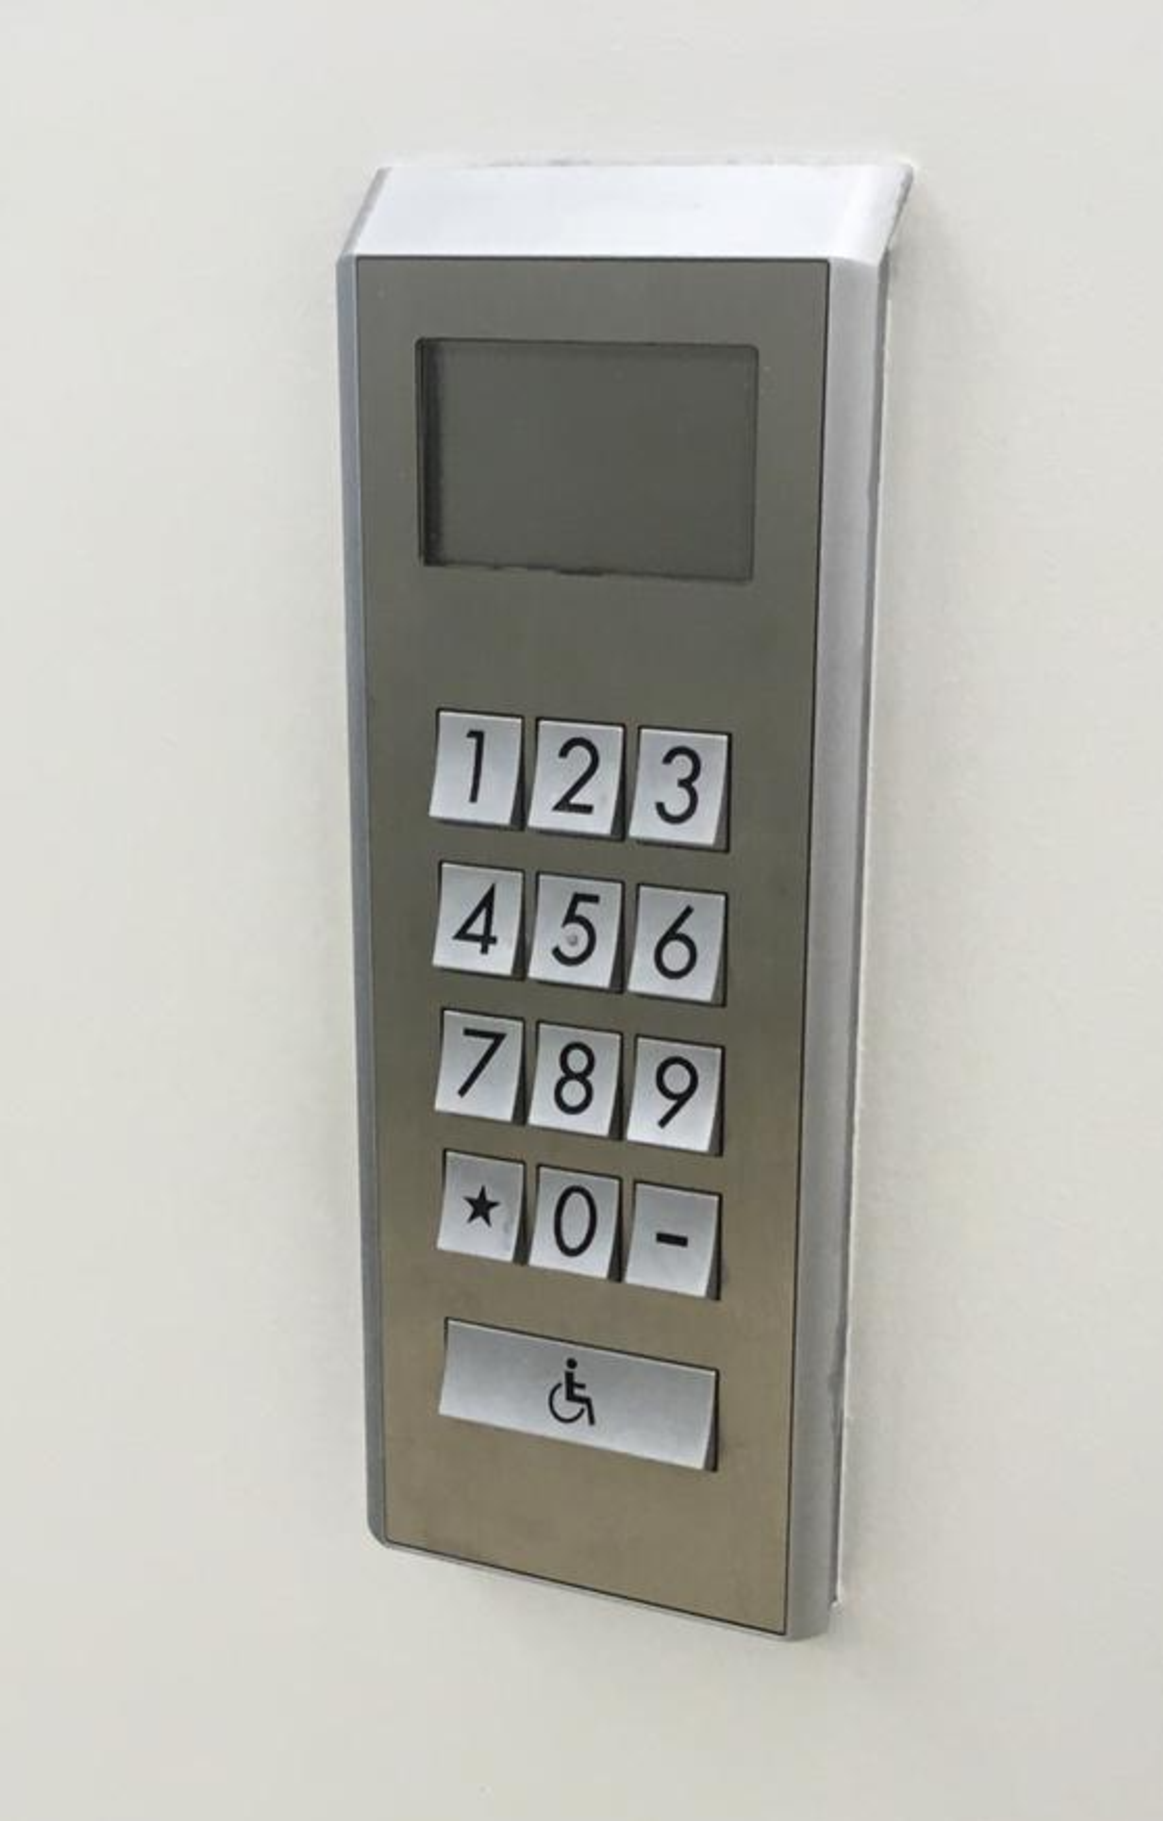
\includegraphics[width=0.40\linewidth]{images/amsovaltower/liftknoppen}
	\caption{Press the floor number(s) and wait for the display to tell you which elevator to get into. It's the smartest elevator system, it's true!}
\end{figure}

\section{The Hague, Central Station}

Added by Jeroen Harmsen: I've reserved a private meeting room in The Hague and Amsterdam, price is 28.35 per person per morning/afternoon (so 56 euro's for a 2 person meeting), incl. coffee, tea, etc.

% If you want to add more experience to this, just add another '\section{City, Location}' in this chapter for reports. All tips are welcome!

\end{document}